% Created by tikzDevice version 0.12.6 on 2026-07-04 06:01:34
% !TEX encoding = UTF-8 Unicode
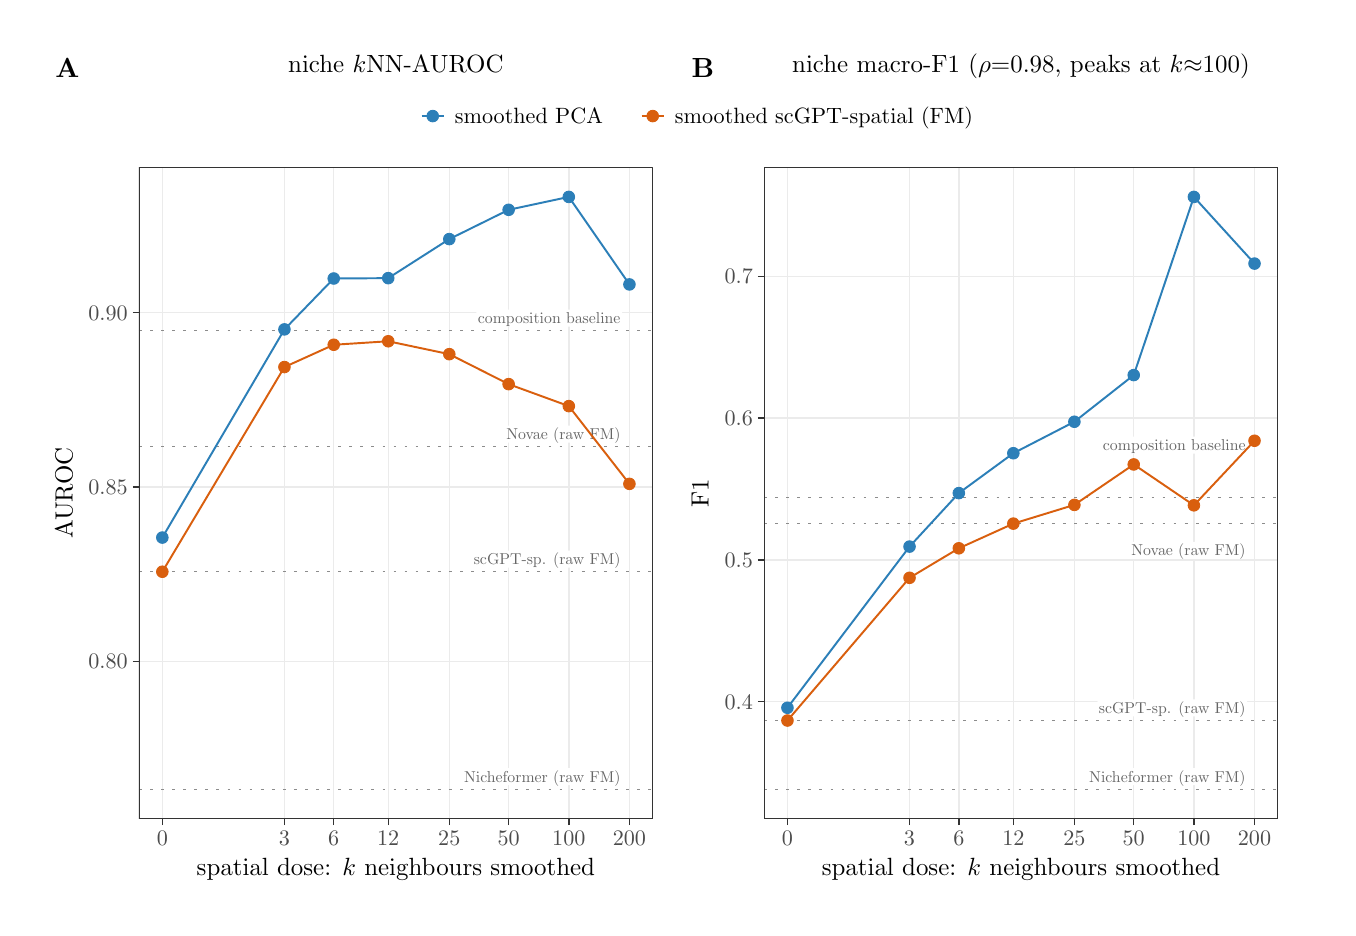
\begin{tikzpicture}[x=1pt,y=1pt]
\definecolor{fillColor}{RGB}{255,255,255}
\path[use as bounding box,fill=fillColor,fill opacity=0.00] (0,0) rectangle (469.75,317.99);
\begin{scope}
\path[clip] (  0.00,  0.00) rectangle (469.75,317.99);
\definecolor{drawColor}{RGB}{255,255,255}
\definecolor{fillColor}{RGB}{255,255,255}

\path[draw=drawColor,line width= 0.5pt,line join=round,line cap=round,fill=fillColor] (  0.00, -0.00) rectangle (469.75,317.99);
\end{scope}
\begin{scope}
\path[clip] (  5.00,  5.00) rectangle (234.88,312.99);
\definecolor{drawColor}{RGB}{255,255,255}
\definecolor{fillColor}{RGB}{255,255,255}

\path[draw=drawColor,line width= 0.5pt,line join=round,line cap=round,fill=fillColor] (  5.00,  5.00) rectangle (234.88,312.99);
\end{scope}
\begin{scope}
\path[clip] (234.88,  5.00) rectangle (460.75,312.99);
\definecolor{drawColor}{RGB}{255,255,255}
\definecolor{fillColor}{RGB}{255,255,255}

\path[draw=drawColor,line width= 0.5pt,line join=round,line cap=round,fill=fillColor] (234.88,  5.00) rectangle (460.75,312.99);
\end{scope}
\begin{scope}
\path[clip] ( 40.22, 32.07) rectangle (225.88,267.54);
\definecolor{fillColor}{RGB}{255,255,255}

\path[fill=fillColor] ( 40.22, 32.07) rectangle (225.88,267.54);
\definecolor{drawColor}{gray}{0.92}

\path[draw=drawColor,line width= 0.5pt,line join=round] ( 40.22, 89.01) --
	(225.88, 89.01);

\path[draw=drawColor,line width= 0.5pt,line join=round] ( 40.22,152.01) --
	(225.88,152.01);

\path[draw=drawColor,line width= 0.5pt,line join=round] ( 40.22,215.00) --
	(225.88,215.00);

\path[draw=drawColor,line width= 0.5pt,line join=round] ( 48.66, 32.07) --
	( 48.66,267.54);

\path[draw=drawColor,line width= 0.5pt,line join=round] ( 92.78, 32.07) --
	( 92.78,267.54);

\path[draw=drawColor,line width= 0.5pt,line join=round] (110.59, 32.07) --
	(110.59,267.54);

\path[draw=drawColor,line width= 0.5pt,line join=round] (130.29, 32.07) --
	(130.29,267.54);

\path[draw=drawColor,line width= 0.5pt,line join=round] (152.35, 32.07) --
	(152.35,267.54);

\path[draw=drawColor,line width= 0.5pt,line join=round] (173.79, 32.07) --
	(173.79,267.54);

\path[draw=drawColor,line width= 0.5pt,line join=round] (195.54, 32.07) --
	(195.54,267.54);

\path[draw=drawColor,line width= 0.5pt,line join=round] (217.44, 32.07) --
	(217.44,267.54);
\definecolor{drawColor}{gray}{0.55}

\path[draw=drawColor,line width= 0.4pt,dash pattern=on 1pt off 3pt ,line join=round] ( 40.22,166.50) -- (225.88,166.50);

\path[draw=drawColor,line width= 0.4pt,dash pattern=on 1pt off 3pt ,line join=round] ( 40.22,121.39) -- (225.88,121.39);

\path[draw=drawColor,line width= 0.4pt,dash pattern=on 1pt off 3pt ,line join=round] ( 40.22, 42.77) -- (225.88, 42.77);

\path[draw=drawColor,line width= 0.4pt,dash pattern=on 1pt off 3pt ,line join=round] ( 40.22,208.45) -- (225.88,208.45);

\path[fill=fillColor] (173.43,168.03) --
	(213.77,168.03) --
	(213.73,168.03) --
	(213.89,168.04) --
	(214.06,168.07) --
	(214.21,168.13) --
	(214.35,168.21) --
	(214.48,168.32) --
	(214.59,168.44) --
	(214.68,168.58) --
	(214.75,168.73) --
	(214.79,168.89) --
	(214.80,169.06) --
	(214.80,169.06) --
	(214.80,173.14) --
	(214.80,173.14) --
	(214.79,173.30) --
	(214.75,173.46) --
	(214.68,173.61) --
	(214.59,173.75) --
	(214.48,173.88) --
	(214.35,173.98) --
	(214.21,174.06) --
	(214.06,174.12) --
	(213.89,174.16) --
	(213.77,174.16) --
	(173.43,174.16) --
	(173.55,174.16) --
	(173.39,174.16) --
	(173.22,174.14) --
	(173.06,174.10) --
	(172.92,174.03) --
	(172.78,173.93) --
	(172.66,173.82) --
	(172.56,173.68) --
	(172.48,173.54) --
	(172.43,173.38) --
	(172.40,173.22) --
	(172.40,173.14) --
	(172.40,169.06) --
	(172.40,169.14) --
	(172.40,168.98) --
	(172.43,168.81) --
	(172.48,168.66) --
	(172.56,168.51) --
	(172.66,168.38) --
	(172.78,168.26) --
	(172.92,168.17) --
	(173.06,168.10) --
	(173.22,168.05) --
	(173.39,168.03) --
	cycle;
\end{scope}
\begin{scope}
\path[clip] ( 40.22, 32.07) rectangle (225.88,267.54);
\definecolor{drawColor}{gray}{0.40}

\node[text=drawColor,anchor=base east,inner sep=0pt, outer sep=0pt, scale=  0.57] at (214.20,169.14) {Novae (raw FM)};
\end{scope}
\begin{scope}
\path[clip] ( 40.22, 32.07) rectangle (225.88,267.54);
\definecolor{fillColor}{RGB}{255,255,255}

\path[fill=fillColor] (161.71,122.92) --
	(213.77,122.92) --
	(213.73,122.92) --
	(213.89,122.93) --
	(214.06,122.96) --
	(214.21,123.02) --
	(214.35,123.11) --
	(214.48,123.21) --
	(214.59,123.33) --
	(214.68,123.47) --
	(214.75,123.63) --
	(214.79,123.79) --
	(214.80,123.95) --
	(214.80,123.95) --
	(214.80,128.03) --
	(214.80,128.03) --
	(214.79,128.19) --
	(214.75,128.35) --
	(214.68,128.51) --
	(214.59,128.65) --
	(214.48,128.77) --
	(214.35,128.88) --
	(214.21,128.96) --
	(214.06,129.02) --
	(213.89,129.05) --
	(213.77,129.06) --
	(161.71,129.06) --
	(161.83,129.05) --
	(161.67,129.06) --
	(161.50,129.04) --
	(161.34,128.99) --
	(161.19,128.92) --
	(161.06,128.83) --
	(160.94,128.71) --
	(160.84,128.58) --
	(160.76,128.43) --
	(160.71,128.28) --
	(160.68,128.11) --
	(160.68,128.03) --
	(160.68,123.95) --
	(160.68,124.03) --
	(160.68,123.87) --
	(160.71,123.71) --
	(160.76,123.55) --
	(160.84,123.40) --
	(160.94,123.27) --
	(161.06,123.16) --
	(161.19,123.06) --
	(161.34,122.99) --
	(161.50,122.94) --
	(161.67,122.92) --
	cycle;
\end{scope}
\begin{scope}
\path[clip] ( 40.22, 32.07) rectangle (225.88,267.54);
\definecolor{drawColor}{gray}{0.40}

\node[text=drawColor,anchor=base east,inner sep=0pt, outer sep=0pt, scale=  0.57] at (214.20,124.03) {scGPT-sp. (raw FM)};
\end{scope}
\begin{scope}
\path[clip] ( 40.22, 32.07) rectangle (225.88,267.54);
\definecolor{fillColor}{RGB}{255,255,255}

\path[fill=fillColor] (158.22, 44.30) --
	(213.77, 44.30) --
	(213.73, 44.30) --
	(213.89, 44.31) --
	(214.06, 44.34) --
	(214.21, 44.40) --
	(214.35, 44.48) --
	(214.48, 44.59) --
	(214.59, 44.71) --
	(214.68, 44.85) --
	(214.75, 45.01) --
	(214.79, 45.17) --
	(214.80, 45.33) --
	(214.80, 45.33) --
	(214.80, 49.41) --
	(214.80, 49.41) --
	(214.79, 49.57) --
	(214.75, 49.73) --
	(214.68, 49.89) --
	(214.59, 50.03) --
	(214.48, 50.15) --
	(214.35, 50.25) --
	(214.21, 50.34) --
	(214.06, 50.40) --
	(213.89, 50.43) --
	(213.77, 50.44) --
	(158.22, 50.44) --
	(158.35, 50.43) --
	(158.18, 50.44) --
	(158.02, 50.42) --
	(157.86, 50.37) --
	(157.71, 50.30) --
	(157.57, 50.20) --
	(157.45, 50.09) --
	(157.35, 49.96) --
	(157.28, 49.81) --
	(157.22, 49.65) --
	(157.20, 49.49) --
	(157.19, 49.41) --
	(157.19, 45.33) --
	(157.20, 45.41) --
	(157.20, 45.25) --
	(157.22, 45.09) --
	(157.28, 44.93) --
	(157.35, 44.78) --
	(157.45, 44.65) --
	(157.57, 44.53) --
	(157.71, 44.44) --
	(157.86, 44.37) --
	(158.02, 44.32) --
	(158.18, 44.30) --
	cycle;
\end{scope}
\begin{scope}
\path[clip] ( 40.22, 32.07) rectangle (225.88,267.54);
\definecolor{drawColor}{gray}{0.40}

\node[text=drawColor,anchor=base east,inner sep=0pt, outer sep=0pt, scale=  0.57] at (214.20, 45.41) {Nicheformer (raw FM)};
\end{scope}
\begin{scope}
\path[clip] ( 40.22, 32.07) rectangle (225.88,267.54);
\definecolor{fillColor}{RGB}{255,255,255}

\path[fill=fillColor] (163.19,209.99) --
	(213.77,209.99) --
	(213.73,209.99) --
	(213.89,209.99) --
	(214.06,210.03) --
	(214.21,210.09) --
	(214.35,210.17) --
	(214.48,210.27) --
	(214.59,210.40) --
	(214.68,210.54) --
	(214.75,210.69) --
	(214.79,210.85) --
	(214.80,211.01) --
	(214.80,211.01) --
	(214.80,215.09) --
	(214.80,215.09) --
	(214.79,215.26) --
	(214.75,215.42) --
	(214.68,215.57) --
	(214.59,215.71) --
	(214.48,215.83) --
	(214.35,215.94) --
	(214.21,216.02) --
	(214.06,216.08) --
	(213.89,216.11) --
	(213.77,216.12) --
	(163.19,216.12) --
	(163.31,216.11) --
	(163.14,216.12) --
	(162.98,216.10) --
	(162.82,216.05) --
	(162.67,215.98) --
	(162.54,215.89) --
	(162.42,215.77) --
	(162.32,215.64) --
	(162.24,215.49) --
	(162.19,215.34) --
	(162.16,215.17) --
	(162.16,215.09) --
	(162.16,211.01) --
	(162.16,211.10) --
	(162.16,210.93) --
	(162.19,210.77) --
	(162.24,210.61) --
	(162.32,210.46) --
	(162.42,210.33) --
	(162.54,210.22) --
	(162.67,210.12) --
	(162.82,210.05) --
	(162.98,210.01) --
	(163.14,209.99) --
	cycle;
\end{scope}
\begin{scope}
\path[clip] ( 40.22, 32.07) rectangle (225.88,267.54);
\definecolor{drawColor}{gray}{0.40}

\node[text=drawColor,anchor=base east,inner sep=0pt, outer sep=0pt, scale=  0.57] at (214.20,211.09) {composition baseline};
\end{scope}
\begin{scope}
\path[clip] ( 40.22, 32.07) rectangle (225.88,267.54);
\definecolor{drawColor}{RGB}{44,127,184}

\path[draw=drawColor,line width= 0.7pt,line join=round] ( 48.66,133.74) --
	( 92.78,208.96) --
	(110.59,227.35) --
	(130.29,227.48) --
	(152.35,241.59) --
	(173.79,252.17) --
	(195.54,256.83) --
	(217.44,225.21);
\definecolor{drawColor}{RGB}{217,95,14}

\path[draw=drawColor,line width= 0.7pt,line join=round] ( 48.66,121.39) --
	( 92.78,195.35) --
	(110.59,203.41) --
	(130.29,204.67) --
	(152.35,200.01) --
	(173.79,189.18) --
	(195.54,181.24) --
	(217.44,153.14);
\definecolor{drawColor}{RGB}{44,127,184}
\definecolor{fillColor}{RGB}{44,127,184}

\path[draw=drawColor,line width= 0.3pt,line join=round,line cap=round,fill=fillColor] ( 48.66,133.74) circle (  2.11);

\path[draw=drawColor,line width= 0.3pt,line join=round,line cap=round,fill=fillColor] ( 92.78,208.96) circle (  2.11);

\path[draw=drawColor,line width= 0.3pt,line join=round,line cap=round,fill=fillColor] (110.59,227.35) circle (  2.11);

\path[draw=drawColor,line width= 0.3pt,line join=round,line cap=round,fill=fillColor] (130.29,227.48) circle (  2.11);

\path[draw=drawColor,line width= 0.3pt,line join=round,line cap=round,fill=fillColor] (152.35,241.59) circle (  2.11);

\path[draw=drawColor,line width= 0.3pt,line join=round,line cap=round,fill=fillColor] (173.79,252.17) circle (  2.11);

\path[draw=drawColor,line width= 0.3pt,line join=round,line cap=round,fill=fillColor] (195.54,256.83) circle (  2.11);

\path[draw=drawColor,line width= 0.3pt,line join=round,line cap=round,fill=fillColor] (217.44,225.21) circle (  2.11);
\definecolor{drawColor}{RGB}{217,95,14}
\definecolor{fillColor}{RGB}{217,95,14}

\path[draw=drawColor,line width= 0.3pt,line join=round,line cap=round,fill=fillColor] ( 48.66,121.39) circle (  2.11);

\path[draw=drawColor,line width= 0.3pt,line join=round,line cap=round,fill=fillColor] ( 92.78,195.35) circle (  2.11);

\path[draw=drawColor,line width= 0.3pt,line join=round,line cap=round,fill=fillColor] (110.59,203.41) circle (  2.11);

\path[draw=drawColor,line width= 0.3pt,line join=round,line cap=round,fill=fillColor] (130.29,204.67) circle (  2.11);

\path[draw=drawColor,line width= 0.3pt,line join=round,line cap=round,fill=fillColor] (152.35,200.01) circle (  2.11);

\path[draw=drawColor,line width= 0.3pt,line join=round,line cap=round,fill=fillColor] (173.79,189.18) circle (  2.11);

\path[draw=drawColor,line width= 0.3pt,line join=round,line cap=round,fill=fillColor] (195.54,181.24) circle (  2.11);

\path[draw=drawColor,line width= 0.3pt,line join=round,line cap=round,fill=fillColor] (217.44,153.14) circle (  2.11);
\definecolor{drawColor}{gray}{0.20}

\path[draw=drawColor,line width= 0.5pt,line join=round,line cap=round] ( 40.22, 32.07) rectangle (225.88,267.54);
\end{scope}
\begin{scope}
\path[clip] (  0.00,  0.00) rectangle (469.75,317.99);
\definecolor{drawColor}{gray}{0.30}

\node[text=drawColor,anchor=base east,inner sep=0pt, outer sep=0pt, scale=  0.80] at ( 36.17, 86.25) {0.80};

\node[text=drawColor,anchor=base east,inner sep=0pt, outer sep=0pt, scale=  0.80] at ( 36.17,149.25) {0.85};

\node[text=drawColor,anchor=base east,inner sep=0pt, outer sep=0pt, scale=  0.80] at ( 36.17,212.25) {0.90};
\end{scope}
\begin{scope}
\path[clip] (  0.00,  0.00) rectangle (469.75,317.99);
\definecolor{drawColor}{gray}{0.20}

\path[draw=drawColor,line width= 0.5pt,line join=round] ( 37.97, 89.01) --
	( 40.22, 89.01);

\path[draw=drawColor,line width= 0.5pt,line join=round] ( 37.97,152.01) --
	( 40.22,152.01);

\path[draw=drawColor,line width= 0.5pt,line join=round] ( 37.97,215.00) --
	( 40.22,215.00);
\end{scope}
\begin{scope}
\path[clip] (  0.00,  0.00) rectangle (469.75,317.99);
\definecolor{drawColor}{gray}{0.20}

\path[draw=drawColor,line width= 0.5pt,line join=round] ( 48.66, 29.82) --
	( 48.66, 32.07);

\path[draw=drawColor,line width= 0.5pt,line join=round] ( 92.78, 29.82) --
	( 92.78, 32.07);

\path[draw=drawColor,line width= 0.5pt,line join=round] (110.59, 29.82) --
	(110.59, 32.07);

\path[draw=drawColor,line width= 0.5pt,line join=round] (130.29, 29.82) --
	(130.29, 32.07);

\path[draw=drawColor,line width= 0.5pt,line join=round] (152.35, 29.82) --
	(152.35, 32.07);

\path[draw=drawColor,line width= 0.5pt,line join=round] (173.79, 29.82) --
	(173.79, 32.07);

\path[draw=drawColor,line width= 0.5pt,line join=round] (195.54, 29.82) --
	(195.54, 32.07);

\path[draw=drawColor,line width= 0.5pt,line join=round] (217.44, 29.82) --
	(217.44, 32.07);
\end{scope}
\begin{scope}
\path[clip] (  0.00,  0.00) rectangle (469.75,317.99);
\definecolor{drawColor}{gray}{0.30}

\node[text=drawColor,anchor=base,inner sep=0pt, outer sep=0pt, scale=  0.80] at ( 48.66, 22.51) {0};

\node[text=drawColor,anchor=base,inner sep=0pt, outer sep=0pt, scale=  0.80] at ( 92.78, 22.51) {3};

\node[text=drawColor,anchor=base,inner sep=0pt, outer sep=0pt, scale=  0.80] at (110.59, 22.51) {6};

\node[text=drawColor,anchor=base,inner sep=0pt, outer sep=0pt, scale=  0.80] at (130.29, 22.51) {12};

\node[text=drawColor,anchor=base,inner sep=0pt, outer sep=0pt, scale=  0.80] at (152.35, 22.51) {25};

\node[text=drawColor,anchor=base,inner sep=0pt, outer sep=0pt, scale=  0.80] at (173.79, 22.51) {50};

\node[text=drawColor,anchor=base,inner sep=0pt, outer sep=0pt, scale=  0.80] at (195.54, 22.51) {100};

\node[text=drawColor,anchor=base,inner sep=0pt, outer sep=0pt, scale=  0.80] at (217.44, 22.51) {200};
\end{scope}
\begin{scope}
\path[clip] (  0.00,  0.00) rectangle (469.75,317.99);
\definecolor{drawColor}{RGB}{0,0,0}

\node[text=drawColor,anchor=base,inner sep=0pt, outer sep=0pt, scale=  0.90] at (133.05, 11.75) {spatial dose: $k$ neighbours smoothed};
\end{scope}
\begin{scope}
\path[clip] (  0.00,  0.00) rectangle (469.75,317.99);
\definecolor{drawColor}{RGB}{0,0,0}

\node[text=drawColor,rotate= 90.00,anchor=base,inner sep=0pt, outer sep=0pt, scale=  0.90] at ( 16.20,149.80) {AUROC};
\end{scope}
\begin{scope}
\path[clip] (  0.00,  0.00) rectangle (469.75,317.99);
\definecolor{drawColor}{RGB}{0,0,0}

\node[text=drawColor,anchor=base,inner sep=0pt, outer sep=0pt, scale=  0.90] at (133.05,301.79) {niche $k$NN-AUROC};
\end{scope}
\begin{scope}
\path[clip] (  0.00,  0.00) rectangle (469.75,317.99);
\definecolor{drawColor}{RGB}{0,0,0}

\node[text=drawColor,anchor=base,inner sep=0pt, outer sep=0pt, scale=  1.00] at ( 14.35,300.03) {\bfseries A};
\end{scope}
\begin{scope}
\path[clip] (266.10, 32.07) rectangle (451.76,267.54);
\definecolor{fillColor}{RGB}{255,255,255}

\path[fill=fillColor] (266.10, 32.07) rectangle (451.75,267.54);
\definecolor{drawColor}{gray}{0.92}

\path[draw=drawColor,line width= 0.5pt,line join=round] (266.10, 74.40) --
	(451.76, 74.40);

\path[draw=drawColor,line width= 0.5pt,line join=round] (266.10,125.66) --
	(451.76,125.66);

\path[draw=drawColor,line width= 0.5pt,line join=round] (266.10,176.92) --
	(451.76,176.92);

\path[draw=drawColor,line width= 0.5pt,line join=round] (266.10,228.18) --
	(451.76,228.18);

\path[draw=drawColor,line width= 0.5pt,line join=round] (274.54, 32.07) --
	(274.54,267.54);

\path[draw=drawColor,line width= 0.5pt,line join=round] (318.66, 32.07) --
	(318.66,267.54);

\path[draw=drawColor,line width= 0.5pt,line join=round] (336.47, 32.07) --
	(336.47,267.54);

\path[draw=drawColor,line width= 0.5pt,line join=round] (356.17, 32.07) --
	(356.17,267.54);

\path[draw=drawColor,line width= 0.5pt,line join=round] (378.23, 32.07) --
	(378.23,267.54);

\path[draw=drawColor,line width= 0.5pt,line join=round] (399.67, 32.07) --
	(399.67,267.54);

\path[draw=drawColor,line width= 0.5pt,line join=round] (421.41, 32.07) --
	(421.41,267.54);

\path[draw=drawColor,line width= 0.5pt,line join=round] (443.32, 32.07) --
	(443.32,267.54);
\definecolor{drawColor}{gray}{0.55}

\path[draw=drawColor,line width= 0.4pt,dash pattern=on 1pt off 3pt ,line join=round] (266.10,138.83) -- (451.76,138.83);

\path[draw=drawColor,line width= 0.4pt,dash pattern=on 1pt off 3pt ,line join=round] (266.10, 67.63) -- (451.76, 67.63);

\path[draw=drawColor,line width= 0.4pt,dash pattern=on 1pt off 3pt ,line join=round] (266.10, 42.77) -- (451.76, 42.77);

\path[draw=drawColor,line width= 0.4pt,dash pattern=on 1pt off 3pt ,line join=round] (266.10,148.16) -- (451.76,148.16);

\path[fill=fillColor] (399.31,126.01) --
	(439.65,126.01) --
	(439.61,126.01) --
	(439.77,126.02) --
	(439.93,126.05) --
	(440.09,126.11) --
	(440.23,126.19) --
	(440.36,126.30) --
	(440.47,126.42) --
	(440.56,126.56) --
	(440.62,126.72) --
	(440.66,126.88) --
	(440.68,127.04) --
	(440.68,127.04) --
	(440.68,131.12) --
	(440.68,131.12) --
	(440.66,131.28) --
	(440.62,131.44) --
	(440.56,131.60) --
	(440.47,131.74) --
	(440.36,131.86) --
	(440.23,131.96) --
	(440.09,132.05) --
	(439.93,132.11) --
	(439.77,132.14) --
	(439.65,132.15) --
	(399.31,132.15) --
	(399.43,132.14) --
	(399.27,132.15) --
	(399.10,132.13) --
	(398.94,132.08) --
	(398.79,132.01) --
	(398.66,131.91) --
	(398.54,131.80) --
	(398.44,131.67) --
	(398.36,131.52) --
	(398.31,131.36) --
	(398.28,131.20) --
	(398.28,131.12) --
	(398.28,127.04) --
	(398.28,127.12) --
	(398.28,126.96) --
	(398.31,126.79) --
	(398.36,126.64) --
	(398.44,126.49) --
	(398.54,126.36) --
	(398.66,126.24) --
	(398.79,126.15) --
	(398.94,126.08) --
	(399.10,126.03) --
	(399.27,126.01) --
	cycle;
\end{scope}
\begin{scope}
\path[clip] (266.10, 32.07) rectangle (451.76,267.54);
\definecolor{drawColor}{gray}{0.40}

\node[text=drawColor,anchor=base east,inner sep=0pt, outer sep=0pt, scale=  0.57] at (440.08,127.12) {Novae (raw FM)};
\end{scope}
\begin{scope}
\path[clip] (266.10, 32.07) rectangle (451.76,267.54);
\definecolor{fillColor}{RGB}{255,255,255}

\path[fill=fillColor] (387.59, 69.16) --
	(439.65, 69.16) --
	(439.61, 69.17) --
	(439.77, 69.17) --
	(439.93, 69.21) --
	(440.09, 69.26) --
	(440.23, 69.35) --
	(440.36, 69.45) --
	(440.47, 69.57) --
	(440.56, 69.71) --
	(440.62, 69.87) --
	(440.66, 70.03) --
	(440.68, 70.19) --
	(440.68, 70.19) --
	(440.68, 74.27) --
	(440.68, 74.27) --
	(440.66, 74.43) --
	(440.62, 74.60) --
	(440.56, 74.75) --
	(440.47, 74.89) --
	(440.36, 75.01) --
	(440.23, 75.12) --
	(440.09, 75.20) --
	(439.93, 75.26) --
	(439.77, 75.29) --
	(439.65, 75.30) --
	(387.59, 75.30) --
	(387.71, 75.29) --
	(387.54, 75.30) --
	(387.38, 75.28) --
	(387.22, 75.23) --
	(387.07, 75.16) --
	(386.94, 75.07) --
	(386.82, 74.95) --
	(386.72, 74.82) --
	(386.64, 74.67) --
	(386.59, 74.52) --
	(386.56, 74.35) --
	(386.56, 74.27) --
	(386.56, 70.19) --
	(386.56, 70.28) --
	(386.56, 70.11) --
	(386.59, 69.95) --
	(386.64, 69.79) --
	(386.72, 69.64) --
	(386.82, 69.51) --
	(386.94, 69.40) --
	(387.07, 69.30) --
	(387.22, 69.23) --
	(387.38, 69.19) --
	(387.54, 69.17) --
	cycle;
\end{scope}
\begin{scope}
\path[clip] (266.10, 32.07) rectangle (451.76,267.54);
\definecolor{drawColor}{gray}{0.40}

\node[text=drawColor,anchor=base east,inner sep=0pt, outer sep=0pt, scale=  0.57] at (440.08, 70.27) {scGPT-sp. (raw FM)};
\end{scope}
\begin{scope}
\path[clip] (266.10, 32.07) rectangle (451.76,267.54);
\definecolor{fillColor}{RGB}{255,255,255}

\path[fill=fillColor] (384.10, 44.30) --
	(439.65, 44.30) --
	(439.61, 44.30) --
	(439.77, 44.31) --
	(439.93, 44.34) --
	(440.09, 44.40) --
	(440.23, 44.48) --
	(440.36, 44.59) --
	(440.47, 44.71) --
	(440.56, 44.85) --
	(440.62, 45.01) --
	(440.66, 45.17) --
	(440.68, 45.33) --
	(440.68, 45.33) --
	(440.68, 49.41) --
	(440.68, 49.41) --
	(440.66, 49.57) --
	(440.62, 49.73) --
	(440.56, 49.89) --
	(440.47, 50.03) --
	(440.36, 50.15) --
	(440.23, 50.25) --
	(440.09, 50.34) --
	(439.93, 50.40) --
	(439.77, 50.43) --
	(439.65, 50.44) --
	(384.10, 50.44) --
	(384.22, 50.43) --
	(384.06, 50.44) --
	(383.89, 50.42) --
	(383.73, 50.37) --
	(383.59, 50.30) --
	(383.45, 50.20) --
	(383.33, 50.09) --
	(383.23, 49.96) --
	(383.15, 49.81) --
	(383.10, 49.65) --
	(383.07, 49.49) --
	(383.07, 49.41) --
	(383.07, 45.33) --
	(383.07, 45.41) --
	(383.07, 45.25) --
	(383.10, 45.09) --
	(383.15, 44.93) --
	(383.23, 44.78) --
	(383.33, 44.65) --
	(383.45, 44.53) --
	(383.59, 44.44) --
	(383.73, 44.37) --
	(383.89, 44.32) --
	(384.06, 44.30) --
	cycle;
\end{scope}
\begin{scope}
\path[clip] (266.10, 32.07) rectangle (451.76,267.54);
\definecolor{drawColor}{gray}{0.40}

\node[text=drawColor,anchor=base east,inner sep=0pt, outer sep=0pt, scale=  0.57] at (440.08, 45.41) {Nicheformer (raw FM)};
\end{scope}
\begin{scope}
\path[clip] (266.10, 32.07) rectangle (451.76,267.54);
\definecolor{fillColor}{RGB}{255,255,255}

\path[fill=fillColor] (389.06,164.05) --
	(439.65,164.05) --
	(439.61,164.05) --
	(439.77,164.06) --
	(439.93,164.09) --
	(440.09,164.15) --
	(440.23,164.23) --
	(440.36,164.34) --
	(440.47,164.46) --
	(440.56,164.60) --
	(440.62,164.75) --
	(440.66,164.91) --
	(440.68,165.08) --
	(440.68,165.08) --
	(440.68,169.15) --
	(440.68,169.15) --
	(440.66,169.32) --
	(440.62,169.48) --
	(440.56,169.63) --
	(440.47,169.77) --
	(440.36,169.90) --
	(440.23,170.00) --
	(440.09,170.08) --
	(439.93,170.14) --
	(439.77,170.17) --
	(439.65,170.18) --
	(389.06,170.18) --
	(389.19,170.17) --
	(389.02,170.18) --
	(388.86,170.16) --
	(388.70,170.12) --
	(388.55,170.04) --
	(388.41,169.95) --
	(388.29,169.84) --
	(388.19,169.70) --
	(388.12,169.56) --
	(388.07,169.40) --
	(388.04,169.24) --
	(388.04,169.15) --
	(388.04,165.08) --
	(388.04,165.16) --
	(388.04,164.99) --
	(388.07,164.83) --
	(388.12,164.67) --
	(388.19,164.53) --
	(388.29,164.39) --
	(388.41,164.28) --
	(388.55,164.19) --
	(388.70,164.12) --
	(388.86,164.07) --
	(389.02,164.05) --
	cycle;
\end{scope}
\begin{scope}
\path[clip] (266.10, 32.07) rectangle (451.76,267.54);
\definecolor{drawColor}{gray}{0.40}

\node[text=drawColor,anchor=base east,inner sep=0pt, outer sep=0pt, scale=  0.57] at (440.08,165.15) {composition baseline};
\end{scope}
\begin{scope}
\path[clip] (266.10, 32.07) rectangle (451.76,267.54);
\definecolor{drawColor}{RGB}{44,127,184}

\path[draw=drawColor,line width= 0.7pt,line join=round] (274.54, 72.24) --
	(318.66,130.48) --
	(336.47,149.80) --
	(356.17,164.21) --
	(378.23,175.59) --
	(399.67,192.45) --
	(421.41,256.83) --
	(443.32,232.74);
\definecolor{drawColor}{RGB}{217,95,14}

\path[draw=drawColor,line width= 0.7pt,line join=round] (274.54, 67.63) --
	(318.66,119.20) --
	(336.47,129.86) --
	(356.17,138.78) --
	(378.23,145.55) --
	(399.67,160.16) --
	(421.41,145.39) --
	(443.32,168.72);
\definecolor{drawColor}{RGB}{44,127,184}
\definecolor{fillColor}{RGB}{44,127,184}

\path[draw=drawColor,line width= 0.3pt,line join=round,line cap=round,fill=fillColor] (274.54, 72.24) circle (  2.11);

\path[draw=drawColor,line width= 0.3pt,line join=round,line cap=round,fill=fillColor] (318.66,130.48) circle (  2.11);

\path[draw=drawColor,line width= 0.3pt,line join=round,line cap=round,fill=fillColor] (336.47,149.80) circle (  2.11);

\path[draw=drawColor,line width= 0.3pt,line join=round,line cap=round,fill=fillColor] (356.17,164.21) circle (  2.11);

\path[draw=drawColor,line width= 0.3pt,line join=round,line cap=round,fill=fillColor] (378.23,175.59) circle (  2.11);

\path[draw=drawColor,line width= 0.3pt,line join=round,line cap=round,fill=fillColor] (399.67,192.45) circle (  2.11);

\path[draw=drawColor,line width= 0.3pt,line join=round,line cap=round,fill=fillColor] (421.41,256.83) circle (  2.11);

\path[draw=drawColor,line width= 0.3pt,line join=round,line cap=round,fill=fillColor] (443.32,232.74) circle (  2.11);
\definecolor{drawColor}{RGB}{217,95,14}
\definecolor{fillColor}{RGB}{217,95,14}

\path[draw=drawColor,line width= 0.3pt,line join=round,line cap=round,fill=fillColor] (274.54, 67.63) circle (  2.11);

\path[draw=drawColor,line width= 0.3pt,line join=round,line cap=round,fill=fillColor] (318.66,119.20) circle (  2.11);

\path[draw=drawColor,line width= 0.3pt,line join=round,line cap=round,fill=fillColor] (336.47,129.86) circle (  2.11);

\path[draw=drawColor,line width= 0.3pt,line join=round,line cap=round,fill=fillColor] (356.17,138.78) circle (  2.11);

\path[draw=drawColor,line width= 0.3pt,line join=round,line cap=round,fill=fillColor] (378.23,145.55) circle (  2.11);

\path[draw=drawColor,line width= 0.3pt,line join=round,line cap=round,fill=fillColor] (399.67,160.16) circle (  2.11);

\path[draw=drawColor,line width= 0.3pt,line join=round,line cap=round,fill=fillColor] (421.41,145.39) circle (  2.11);

\path[draw=drawColor,line width= 0.3pt,line join=round,line cap=round,fill=fillColor] (443.32,168.72) circle (  2.11);
\definecolor{drawColor}{gray}{0.20}

\path[draw=drawColor,line width= 0.5pt,line join=round,line cap=round] (266.10, 32.07) rectangle (451.75,267.54);
\end{scope}
\begin{scope}
\path[clip] (  0.00,  0.00) rectangle (469.75,317.99);
\definecolor{drawColor}{gray}{0.30}

\node[text=drawColor,anchor=base east,inner sep=0pt, outer sep=0pt, scale=  0.80] at (262.05, 71.64) {0.4};

\node[text=drawColor,anchor=base east,inner sep=0pt, outer sep=0pt, scale=  0.80] at (262.05,122.90) {0.5};

\node[text=drawColor,anchor=base east,inner sep=0pt, outer sep=0pt, scale=  0.80] at (262.05,174.16) {0.6};

\node[text=drawColor,anchor=base east,inner sep=0pt, outer sep=0pt, scale=  0.80] at (262.05,225.42) {0.7};
\end{scope}
\begin{scope}
\path[clip] (  0.00,  0.00) rectangle (469.75,317.99);
\definecolor{drawColor}{gray}{0.20}

\path[draw=drawColor,line width= 0.5pt,line join=round] (263.85, 74.40) --
	(266.10, 74.40);

\path[draw=drawColor,line width= 0.5pt,line join=round] (263.85,125.66) --
	(266.10,125.66);

\path[draw=drawColor,line width= 0.5pt,line join=round] (263.85,176.92) --
	(266.10,176.92);

\path[draw=drawColor,line width= 0.5pt,line join=round] (263.85,228.18) --
	(266.10,228.18);
\end{scope}
\begin{scope}
\path[clip] (  0.00,  0.00) rectangle (469.75,317.99);
\definecolor{drawColor}{gray}{0.20}

\path[draw=drawColor,line width= 0.5pt,line join=round] (274.54, 29.82) --
	(274.54, 32.07);

\path[draw=drawColor,line width= 0.5pt,line join=round] (318.66, 29.82) --
	(318.66, 32.07);

\path[draw=drawColor,line width= 0.5pt,line join=round] (336.47, 29.82) --
	(336.47, 32.07);

\path[draw=drawColor,line width= 0.5pt,line join=round] (356.17, 29.82) --
	(356.17, 32.07);

\path[draw=drawColor,line width= 0.5pt,line join=round] (378.23, 29.82) --
	(378.23, 32.07);

\path[draw=drawColor,line width= 0.5pt,line join=round] (399.67, 29.82) --
	(399.67, 32.07);

\path[draw=drawColor,line width= 0.5pt,line join=round] (421.41, 29.82) --
	(421.41, 32.07);

\path[draw=drawColor,line width= 0.5pt,line join=round] (443.32, 29.82) --
	(443.32, 32.07);
\end{scope}
\begin{scope}
\path[clip] (  0.00,  0.00) rectangle (469.75,317.99);
\definecolor{drawColor}{gray}{0.30}

\node[text=drawColor,anchor=base,inner sep=0pt, outer sep=0pt, scale=  0.80] at (274.54, 22.51) {0};

\node[text=drawColor,anchor=base,inner sep=0pt, outer sep=0pt, scale=  0.80] at (318.66, 22.51) {3};

\node[text=drawColor,anchor=base,inner sep=0pt, outer sep=0pt, scale=  0.80] at (336.47, 22.51) {6};

\node[text=drawColor,anchor=base,inner sep=0pt, outer sep=0pt, scale=  0.80] at (356.17, 22.51) {12};

\node[text=drawColor,anchor=base,inner sep=0pt, outer sep=0pt, scale=  0.80] at (378.23, 22.51) {25};

\node[text=drawColor,anchor=base,inner sep=0pt, outer sep=0pt, scale=  0.80] at (399.67, 22.51) {50};

\node[text=drawColor,anchor=base,inner sep=0pt, outer sep=0pt, scale=  0.80] at (421.41, 22.51) {100};

\node[text=drawColor,anchor=base,inner sep=0pt, outer sep=0pt, scale=  0.80] at (443.32, 22.51) {200};
\end{scope}
\begin{scope}
\path[clip] (  0.00,  0.00) rectangle (469.75,317.99);
\definecolor{drawColor}{RGB}{0,0,0}

\node[text=drawColor,anchor=base,inner sep=0pt, outer sep=0pt, scale=  0.90] at (358.93, 11.75) {spatial dose: $k$ neighbours smoothed};
\end{scope}
\begin{scope}
\path[clip] (  0.00,  0.00) rectangle (469.75,317.99);
\definecolor{drawColor}{RGB}{0,0,0}

\node[text=drawColor,rotate= 90.00,anchor=base,inner sep=0pt, outer sep=0pt, scale=  0.90] at (246.08,149.80) {F1};
\end{scope}
\begin{scope}
\path[clip] (  0.00,  0.00) rectangle (469.75,317.99);
\definecolor{drawColor}{RGB}{0,0,0}

\node[text=drawColor,anchor=base,inner sep=0pt, outer sep=0pt, scale=  0.90] at (358.93,301.79) {niche macro-F1 ($\rho{=}0.98$, peaks at $k{\approx}100$)};
\end{scope}
\begin{scope}
\path[clip] (  0.00,  0.00) rectangle (469.75,317.99);
\definecolor{drawColor}{RGB}{0,0,0}

\node[text=drawColor,anchor=base,inner sep=0pt, outer sep=0pt, scale=  1.00] at (243.97,300.03) {\bfseries B};
\end{scope}
\begin{scope}
\path[clip] (  0.00,  0.00) rectangle (469.75,317.99);
\definecolor{fillColor}{RGB}{255,255,255}

\path[fill=fillColor] (136.87,276.54) rectangle (355.11,295.54);
\end{scope}
\begin{scope}
\path[clip] (  0.00,  0.00) rectangle (469.75,317.99);
\definecolor{fillColor}{RGB}{255,255,255}

\path[fill=fillColor] (141.37,281.04) rectangle (151.37,291.04);
\definecolor{drawColor}{RGB}{44,127,184}

\path[draw=drawColor,line width= 0.7pt,line join=round] (142.37,286.04) -- (150.37,286.04);
\definecolor{fillColor}{RGB}{44,127,184}

\path[draw=drawColor,line width= 0.3pt,line join=round,line cap=round,fill=fillColor] (146.37,286.04) circle (  2.11);
\end{scope}
\begin{scope}
\path[clip] (  0.00,  0.00) rectangle (469.75,317.99);
\definecolor{fillColor}{RGB}{255,255,255}

\path[fill=fillColor] (220.86,281.04) rectangle (230.86,291.04);
\definecolor{drawColor}{RGB}{217,95,14}

\path[draw=drawColor,line width= 0.7pt,line join=round] (221.86,286.04) -- (229.86,286.04);
\definecolor{fillColor}{RGB}{217,95,14}

\path[draw=drawColor,line width= 0.3pt,line join=round,line cap=round,fill=fillColor] (225.86,286.04) circle (  2.11);
\end{scope}
\begin{scope}
\path[clip] (  0.00,  0.00) rectangle (469.75,317.99);
\definecolor{drawColor}{RGB}{0,0,0}

\node[text=drawColor,anchor=base west,inner sep=0pt, outer sep=0pt, scale=  0.80] at (154.37,283.28) {smoothed PCA};
\end{scope}
\begin{scope}
\path[clip] (  0.00,  0.00) rectangle (469.75,317.99);
\definecolor{drawColor}{RGB}{0,0,0}

\node[text=drawColor,anchor=base west,inner sep=0pt, outer sep=0pt, scale=  0.80] at (233.86,283.28) {smoothed scGPT-spatial (FM)};
\end{scope}
\end{tikzpicture}
